\documentclass[11pt]{scrartcl}
\usepackage{dominatrix}
\usepackage{solarized-light}
\lstset{
language=R
}

\newcommand{\sgn}{\ensuremath{\mathrm{sgn}}}

\newcommand{\km}{$k$-means}
\newcommand{\defrac}[2]{\ensuremath{\frac{\delta #1}{\delta #2}}}

\usepackage{dsfont}

\title{Homework 4}
\subject{Statistical Machine Learning (STAT W4400)}
\author{Linan Qiu\\\texttt{lq2137}}
\begin{document}
\maketitle

\textbf{As usual, the \texttt{R} code is available at \url{https://github.com/linanqiu/stat-w4400-homework}}

\section{PCA}

\subsection{How many principal components}

Since dimensionality of raw data is 10304, the number of principal components is 10304.

\subsection{Approximately reconstruct a specific face image}

\begin{align*}
\hat{x}_i &= \sum_{j=1}^d \left<\mathbf{x}_i,\xi_j \right> \xi_j\\
&=\sum_{j=1}^d c_{i,j} \xi_j
\end{align*}

where $c_i$ is the projection of $\mathbf{x_i}$ onto $\xi_i$ and $\xi_i$ is the eigenvector corresponding to the $j$-th largest eigenvalue. Dimensionality reduction occurs because instead of storing the complete $\mathbf{x}_i \in \mathbb{R}^{10304}$, we store only $\mathbf{c}_i \in \mathbb{R}^d$ and $d$ eigenvectors $\xi_i \in \mathbb{R}^{10304}$, and usually $d \ll 10304$.

\section{\km}

\subsection{$C_k$ intuition}

$C_k$ is the set of all (indices of) data points assigned to cluster $k$ (ie. $m_i = k$.)

\subsection{Describe the objective}

Breaking down the objective,

\[||x_i - x_j||^2_2\]

is the squared distance between data point $x_i$ and data point $x_j$.

\[\sum_{i \in C_k} \sum_{j \in C_k}||x_i - x_j||^2_2\]

is the sum of squared distances between all possible pairs of data points of $x_i | i \in C_k$, ie. the sum of distances between all data points that are assigned to $k$.

\[\frac{1}{|C_k|} \sum_{i \in C_k} \sum_{j \in C_k}||x_i - x_j||^2_2\]

scales the sum based on the number of elements in $C_k$, giving a measure, for each cluster, of how far apart the data points are from each other. This is also a measure of the mean distance of all data points in $k$ to the cluster center (exact proof of this intuition is the next part of the question).

\[\sum_{k=1}^K \frac{1}{|C_k|} \sum_{i \in C_k} \sum_{j \in C_k}||x_i - x_j||^2_2\]

sums this measure for all clusters $k \in K$, measuring the total mean distance of all data points to their respective cluster centers.

By minimizing this, we minimize the total mean distance of all data points to their cluster centers, effectively finding clustering assignments $\mathbf{m}$ that ``bunches / clusters'' data points closest together in the same group.

\subsection{Prove that $\frac{1}{|C_k|}\sum_{i \in C_k} \sum_{j \in C_k} ||x_i - x_j||^2_2 = 2 \sum_{i\in C_k} ||x_i - \mu_k||^2_2$}

In this step, we are formalizing the intuition earlier that $\frac{1}{|C_k|}\sum_{i \in C_k} \sum_{j \in C_k} ||x_i - x_j||^2_2$ is indeed a measure of the mean distance of all data points in $k$ to the cluster center. 

\begin{align*}
\frac{1}{|C_k|} \sum_{i \in C_k} \sum_{j \in C_k} ||x_i - x_j||^2_2 &= \frac{1}{|C_k|} \sum_{i \in C_k} \sum_{j \in C_k} ||x_i - \mu_k + \mu_k - x_j||^2_2 \\
&= \frac{1}{|C_k|} \sum_{i \in C_k} \sum_{j \in C_k} \left( ||x_i - \mu_k||^2_2 + ||\mu_k - x_j||^2_2 + 2\left<x_i - \mu_k, \mu_k - x_j\right> \right) \\
\end{align*}

For each of the three terms in the round brackets,

\begin{align*}
\frac{1}{|C_k|} \sum_{i \in C_k} \sum_{j \in C_k} ||x_i - \mu_k||^2_2 &= \frac{1}{|C_k|} \sum_{i \in C_k} |C_k| * ||x_i - \mu_k||^2_2 \\
&= \sum_{i \in C_k} ||x_i - \mu_k||^2_2 \\
\frac{1}{|C_k|} \sum_{i \in C_k} \sum_{j \in C_k} ||\mu_k - x_j||^2_2 &= \frac{1}{|C_k|} \sum_{j \in C_k} |C_k| * ||\mu_k - x_j||^2_2 \\
&= \sum_{j \in C_k} ||\mu_k - x_j||^2_2 \\
&= \sum_{i \in C_k} ||\mu_k - x_i||^2_2 \\
&= \sum_{i \in C_k} ||x_i - \mu_k||^2_2 \\
\frac{1}{|C_k|} \sum_{i \in C_k} \sum_{j \in C_k} 2\left<x_i - \mu_k, \mu_k - x_j\right> &= \frac{2}{|C_k|}\sum_{i\in C_k} \left<x_i - \mu_k, \sum_{j \in C_k} (\mu_k - x_j) \right> \\
&= \frac{2}{|C_k|}\sum_{i\in C_k} \left<x_i - \mu_k, 0 \right> \\
&= 0
\end{align*}

Since by definition, $\sum_{j \in C_k} (\mu_k - x_j) = |C_k|\mu_k - \sum_{j \in C_k} x_j = |C-k|\mu_k - |C_k|\mu_k = 0$. Then,

\[\frac{1}{|C_k|} \sum_{i \in C_k} \sum_{j \in C_k} ||x_i - x_j||^2_2 = 2 \sum_{i \in C_k} ||x_i - \mu_k||^2_2\]

\subsection{Prove result implies that the \km algorithm decreases the objective with each step of the algorithm}

Let $\sum_{i \in C_k} ||x_i - \mu_k||^2_2 = \mathrm{RSS}$

\begin{align*}
\defrac{\mathrm{RSS}}{\mu_k} &= \defrac{}{\mu_k} \sum_{i \in C_k} ||x_i - \mu_k||^2_2 \\
&= \defrac{}{\mu_k} \sum_{i \in C_k} \sum_{d=1}^D (x_{i,d} - \mu_{k,d})^2 \\
&= - 2 \sum_{i \in C_k} \sum_{d=1}^D (x_{i,d} - \mu_{k,d}) \\
&= 2 \left[ \sum_{i \in C_k} \sum_{d=1}^D x_{i,d} - \sum_{i \in C_k} \sum_{d=1}^D \mu_{k,d} \right] \\
&= 2 \left[ \sum_{i \in C_k} x_i - \sum_{i \in C_k} \mu_k \right] = 0
\end{align*}

Then,

\begin{align*}
\sum_{i \in C_k} x_i &= \sum_{i \in C_k} \mu_k \\
\sum_{i \in C_k} x_i &= |C_k| \mu_k \\
\mu_k &= \frac{1}{|C_k|} \sum_{i \in C_k} x_i 
\end{align*}

This is the definition of $\mu_k$.

This makes sense, since there are two steps per iteration: reassignment and recomputation. RSS decreases in the reassignment step since each data point is assigned to the closest centroid, so the distance it contributes to the total RSS decreases. Furthermore, it decreases in the recomputation step because the new centroid is the $k$ for which $\mathrm{RSS}_k$ is minimum. As shown above, we minimize $\mathrm{RSS}_k$ when the old centroid is replaced with the new centroid.

\section{Multinomial Clustering}

\subsection{Implement EM algoithm in \texttt{R}}

Done in \texttt{em.R}.

\subsection{Run algorithm on $K \in \{3, 4, 5\}$}

Done in \texttt{run-seq.R}. Produces \texttt{plot3.pdf}, \texttt{plot4.pdf}, \texttt{plot5.pdf}. A parallel version that does the algorithm on different $K$s in parallel is in \texttt{run-par.R}. This was fun \texttt{:D}

\subsection{Visualize the results}

\begin{figure}[H]
\centering
\begin{subfigure}[t]{.3\textwidth}
\centering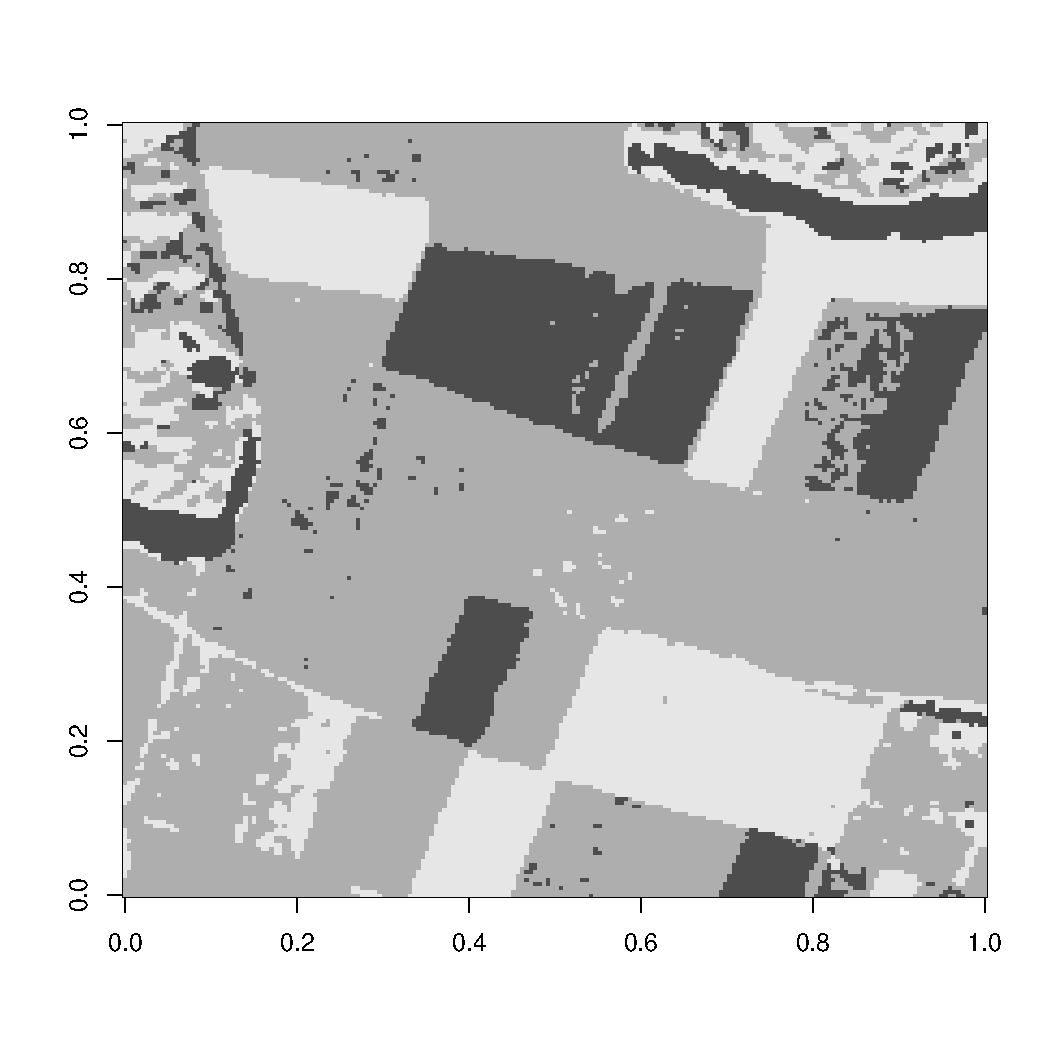
\includegraphics[height=5cm]{./hw4/plot3.pdf}
\caption{Results for $K=3$}
\label{k3}
\end{subfigure}
\begin{subfigure}[t]{.3\textwidth}
\centering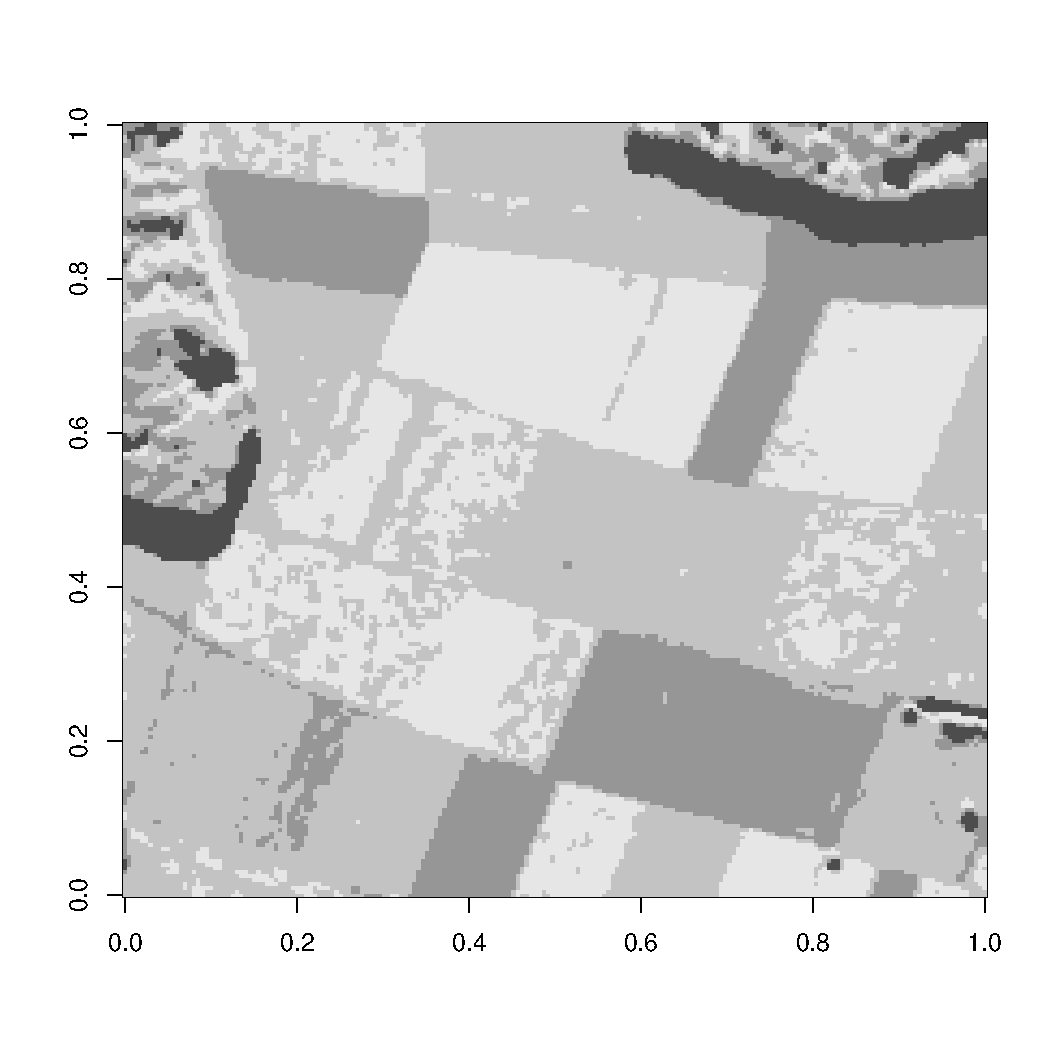
\includegraphics[height=5cm]{./hw4/plot4.pdf}
\caption{Results for $K=4$}
\label{k4}
\end{subfigure}
\begin{subfigure}[t]{.3\textwidth}
\centering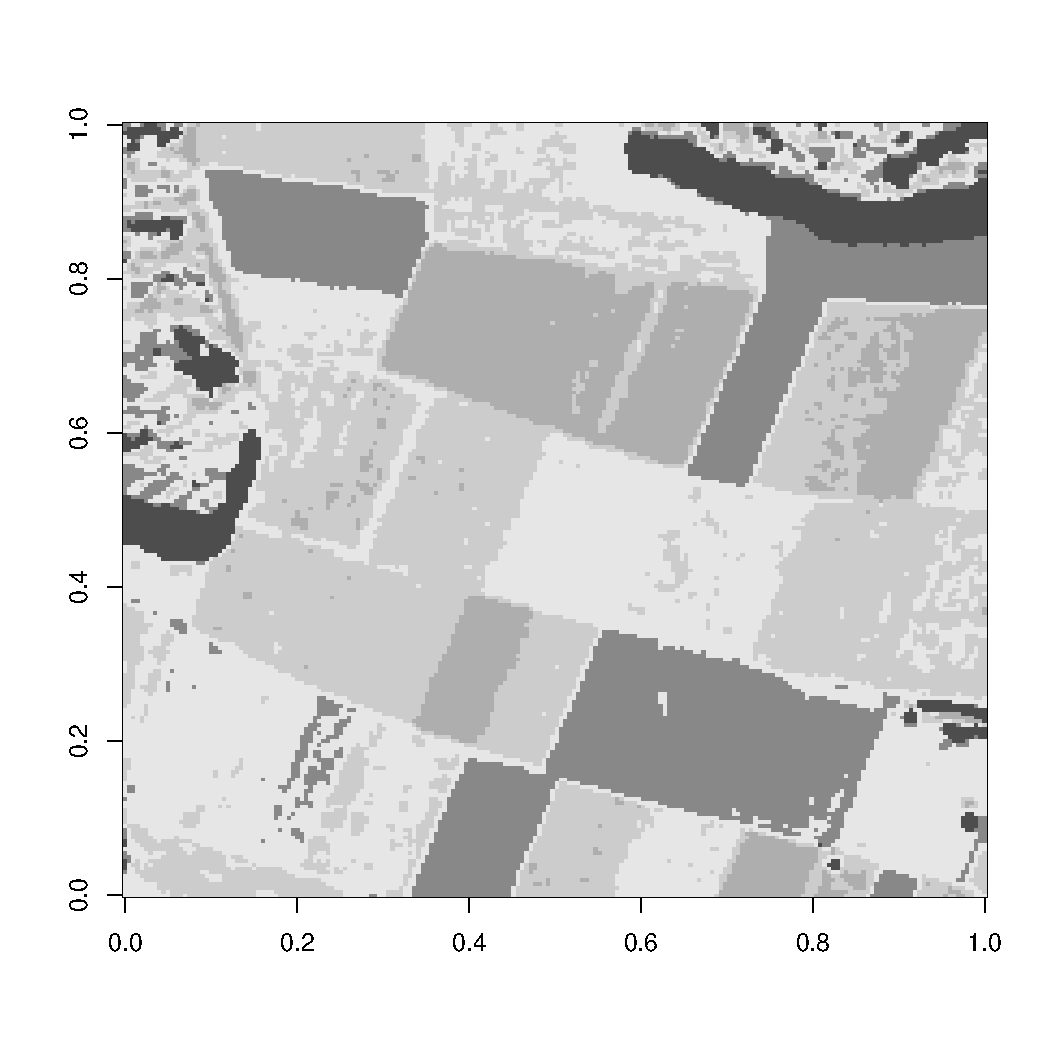
\includegraphics[height=5cm]{./hw4/plot5.pdf}
\caption{Results for $K=5$}
\label{k5}
\end{subfigure}
\caption{Results for histogram cluster for $K \in \{3, 4, 5\}$}
\end{figure}

\end{document}
